\subsection{UC28 - Annullamento dell'ordinazione}\label{usecase:28}
\begin{figure}[H]
    \centering
    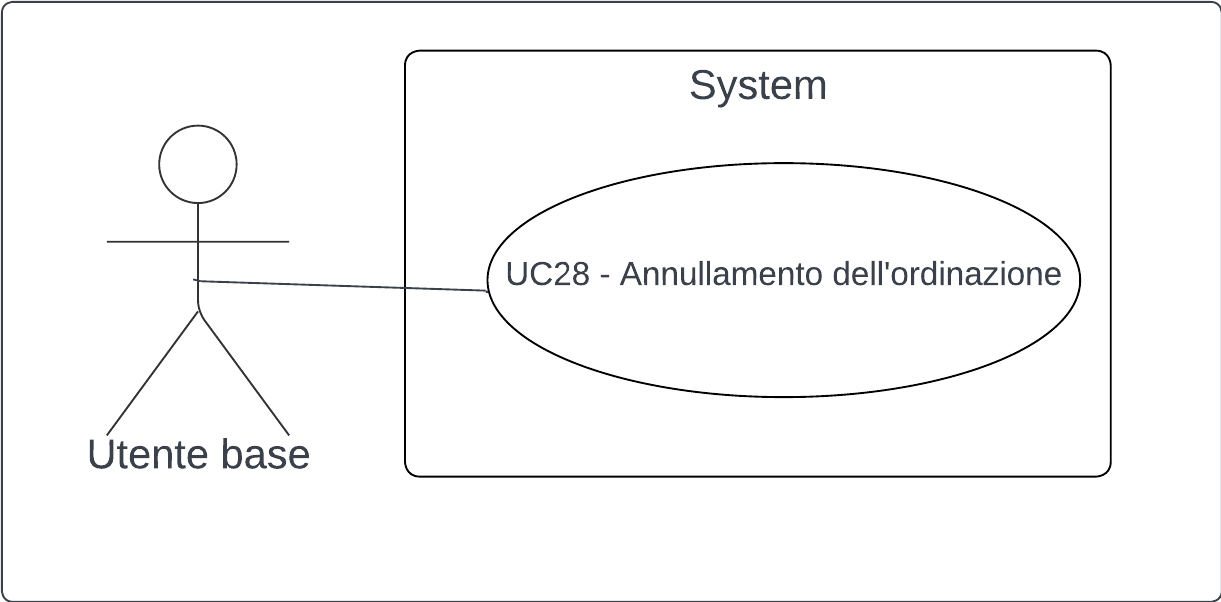
\includegraphics[width=0.9\linewidth]{ucd/UCD28.png}
    \caption{Annullamento dell'ordinazione}
\end{figure}
\textbf{Attori}:
\begin{itemize}
    \item Utente base.
\end{itemize}
\textbf{Precondizioni}:
\begin{itemize}
    \item L'utente ha creato un'ordinazione collaborativa (\nameref{usecase:3});
    \item Il tempo utile per annullare l'ordinazione non è scaduto.
\end{itemize}
\textbf{Postcondizioni}:
\begin{itemize}
    \item Le ordinazioni associate ad un utente della prenotazione collaborativa sono state annullate e ora quell'utente non ha ordinazioni associate.
\end{itemize}
\textbf{Scenario principale}:
\begin{enumerate}
    \item L'utente sceglie l'opzione di annullamento delle ordinazioni;
    \item Il sistema annulla le ordinazioni associate all'utente.
\end{enumerate}
\newpage